\documentclass{article}

\usepackage{pdfpages}

\usepackage[hidelinks]{hyperref}

\usepackage{array}
\usepackage{tabularx}

\usepackage{comment}

\usepackage{tcolorbox}

\usepackage{graphicx}
\usepackage{subcaption}

\usepackage{amsmath}

\usepackage{float}

\usepackage[export]{adjustbox}

\usepackage[margin=1.25in]{geometry}

\newtcbox{\inlinecode}{on line, boxrule=0pt, boxsep=0pt, top=2pt, left=2pt, bottom=2pt, right=2pt, colback=gray!15, colframe=white, fontupper={\ttfamily \footnotesize}}

\begin{document}
\pagenumbering{gobble}

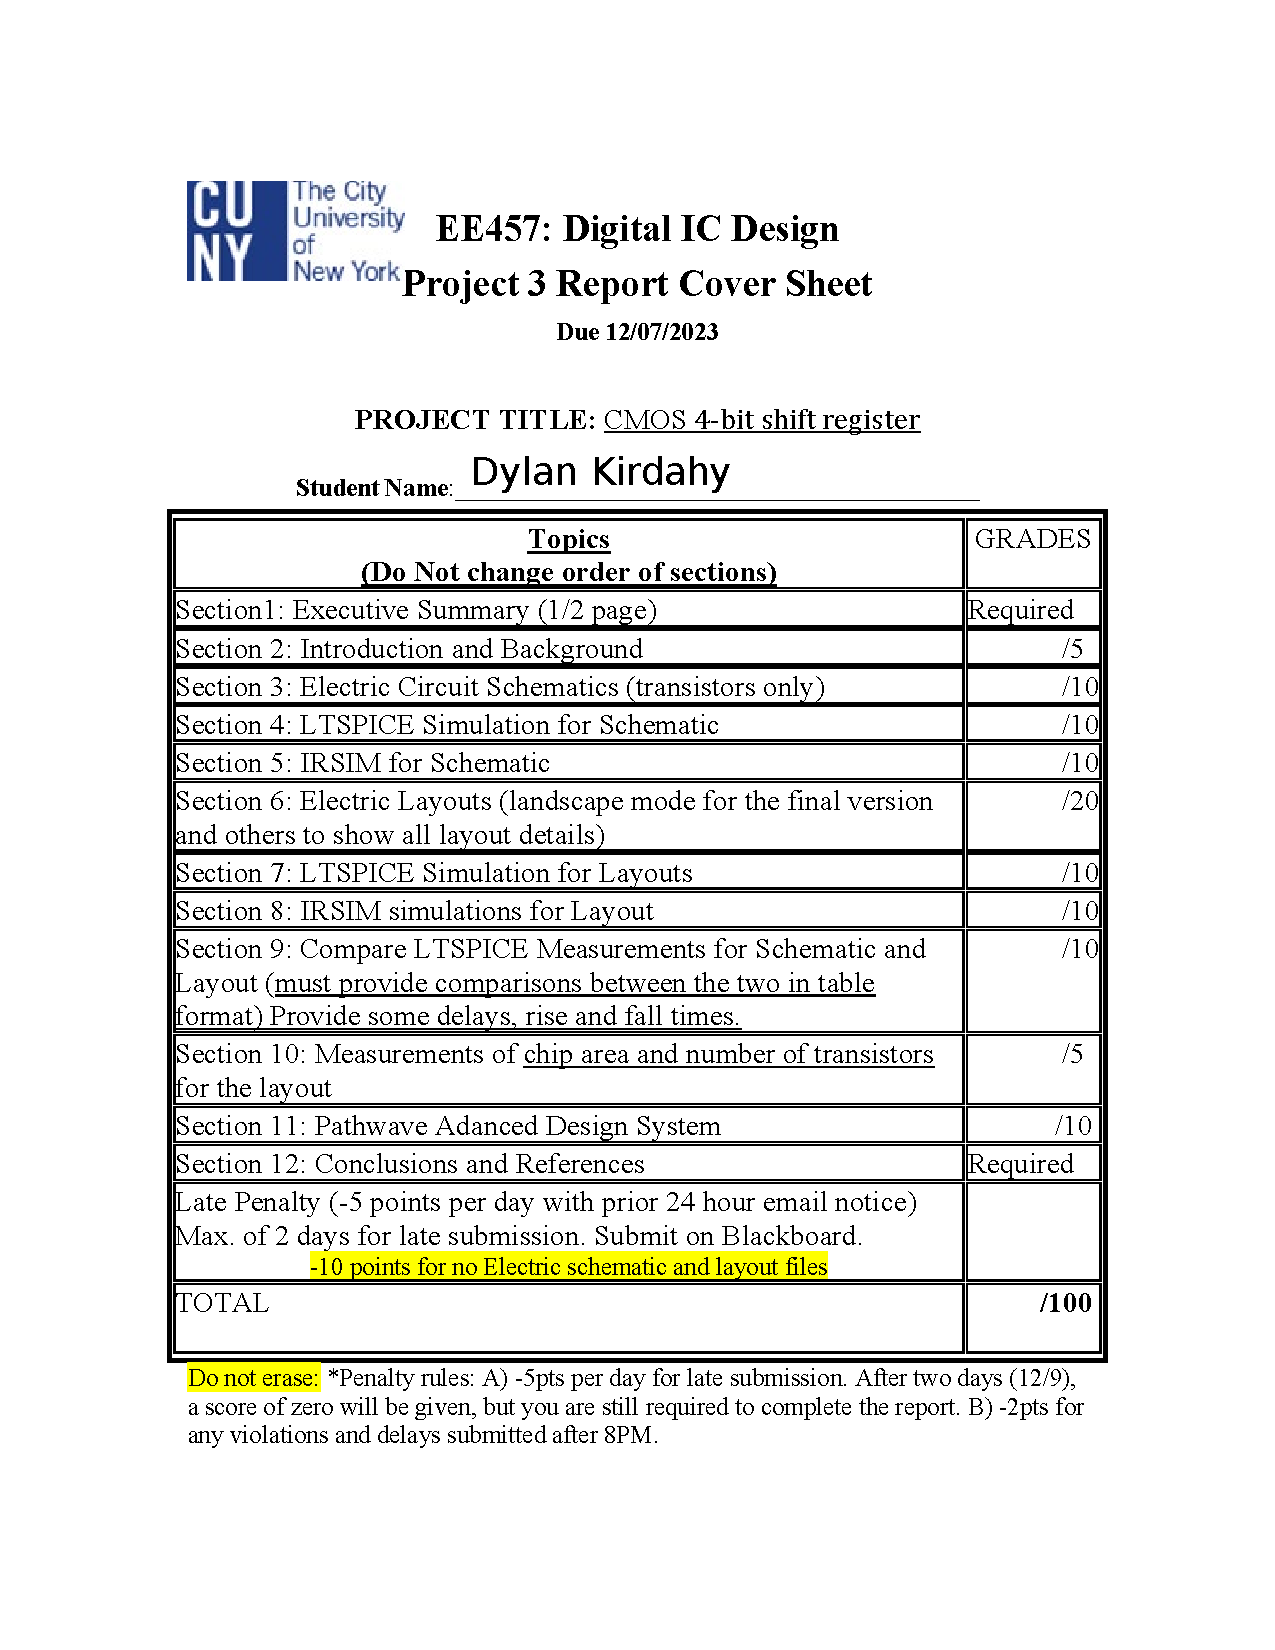
\includepdf[pages=-,scale=1,pagecommand={}]{cover-sheet.pdf}

\tableofcontents

\newpage
\pagenumbering{arabic}

\section{Executive Summary}
  \paragraph{}
  The goal of this project was to build a 4-bit shift register in Electric.  



\newpage
\section{References}

\noindent [\text{1}] EE 457 Lectures 1, 2, 3, and 4

\noindent [\text{2}] https://cmosedu.com/videos/electric/tutorial3/electric\_tutorial\_3.htm 

\noindent [\text{3}] https://cmosedu.com/videos/electric/tutorial4/electric\_tutorial\_4.htm 

\noindent [\text{4}] https://en.wikipedia.org/wiki/Multiplexer

\noindent [\text{5}] https://vlsiuniverse.blogspot.com/search/label/8\%3A1\%20mux

\noindent [\text{6}] https://cmosedu.com/videos/electric/tutorial5/electric\_tutorial\_5.htm 

\end{document}
